\documentclass[a4paper]{scrartcl}
\usepackage[cm]{fullpage}
\usepackage{amsmath, amssymb, esint}
\usepackage{siunitx}
\usepackage{caption}

\usepackage{tikz}

\begin{document}

\title{PHYS2111: Heisenberg Uncertainty}
\author{ \\ \\ }
\date{2016-05-18}
\maketitle

\begin{abstract}
    By measuring the single slit diffraction pattern of \SI{632.8}{\nano\metre} light across a plane, it is found to match reasonably well to the expected Fraunhofer diffraction pattern. It was also determined to be not a good way to test Heisenberg's uncertainty principle.
\end{abstract}

\section{Introduction}
Please refer to the student notes of the experiment.

\section{Materials and Methods}
Please refer to the operating instructions of the experiment.

If each photon has equal probability of passing the slit at any position between the slit (i.e., a uniform distribution of photons at the slit), it's standard deviation is \(\sigma_x = \frac{W}{2 \sqrt{3}}\), where \(W\) is the slit width.

By the uncertainty principle, this means:
\[\sigma_{p_x} \ge \frac{\hbar \sqrt{3}}{W}\]
where \(\sigma_{p_x}\) is the standard deviation of momentum in the \(x\) direction. Let \(P_x\) be a random variable of this distribution.

Taking the (normalised) measured intensities along the \(x\) axis as a probability distribution, let \(X\) be a random variable of this distribution. This can be converted to a \(P_x\) variable by:
\[P_x = \frac{h}{\lambda} \sin \tan^{-1} \frac{X}{z}\]
where \(z\) is the distance from the slit to the detector plane (See derivation in the student notes).

By definition, this means we can calculate \(\sigma_{p_x}\) with:
\[\sigma_{p_x}^2 = \operatorname{E}[(P_x - \operatorname{E}[P_x])^2]\]

For a perfect single slit Fraunhofer diffraction pattern, this is equal to:
\[\sigma_{p_x}^2 = \frac{h^2 z}{\pi^2 \lambda W} \int_{-\infty}^{\infty} \frac{\sin^2 \left(\frac{\pi W x}{\lambda z}\right)}{x^2 + z^2} \:\mathrm{d}x\]

There was a distance of \SI{1.000 \pm 0.005}{\metre} between the slit and detector. The detector was sweeped continuously from one side's third minima to the other side.

Slits labelled \SI{0.1}{\milli\metre}, \SI{0.2}{\milli\metre} and \SI{0.4}{\milli\metre} were used.

\section{Results}
\begin{figure}
    \centering
    \includegraphics[height = 6cm]{{0.1}.png}
    \caption{Intensity of the \SI{0.1}{\milli\metre} slit}
    \label{fig:0.1}
\end{figure}
\begin{figure}
    \centering
    \includegraphics[height = 6cm]{{0.2}.png}
    \caption{\\
        Blue: Intensity of the \SI{0.2}{\milli\metre} slit \\
        Orange: Theoretical pattern for a \SI{0.19}{\milli\metre} slit
    }
    \label{fig:0.2}
\end{figure}
\begin{figure}
    \centering
    \includegraphics[height = 6cm]{{0.4}.png}
    \caption{\\
        Blue: Intensity of the \SI{0.4}{\milli\metre} slit \\
        Orange: Theoretical pattern for a \SI{0.38}{\milli\metre} slit
    }
    \label{fig:0.4}
\end{figure}

\begin{table}
    \centering
    \begin{tabular}{c | c | c}
        Slit Width (\si{\milli\metre}) & Actual \(\sigma_{p_x}\) (\si{h\per\milli\metre}) & Minimum  \(\sigma_{p_x}\) (\si{h\per\milli\metre}) \\
        \hline
        0.1 & \SI{5.6}{} & \SI{17}{} \\
        0.2 & \SI{2.3}{} & \SI{8.7}{} \\
        0.4 & \SI{1.1}{} & \SI{4.3}{}
    \end{tabular}
    \caption{Actual and minimum expected \(\sigma_{p_x}\)}
    \label{tab:momentum-stddev}
\end{table}

\begin{table}
    \centering
    \begin{tabular}{c | c | c}
        Slit Width (\si{\milli\metre}) & Measured (\si{\milli\metre}) & Expected (\si{\milli\metre}) \\
        \hline
        0.1 & \SI{14 \pm 0.5}{} & \SI{12.7 \pm 0.1}{} \\
        0.2 & \SI{6.5 \pm 0.3}{} & \SI{6.33}{} \\
        0.4 & \SI{3.8 \pm 0.1}{} & \SI{3.16}{}
    \end{tabular}
    \caption{Measured and expected distances between minima}
    \label{tab:minima}
\end{table}

The measured diffraction patterns, as well as the fitted Fraunhofer single slit diffraction pattern are shown in Figures \ref{fig:0.1}, \ref{fig:0.2} and \ref{fig:0.4}.

The calculated \(\sigma_{p_x}\) is shown in Table \ref{tab:momentum-stddev}, as well as the minimum expected value by the uncertainty principle.

The distances between minima are shown in Table \ref{tab:minima}, as well as the expected values by the wave theory of light.

\section{Discussion}
\begin{figure}
    \centering
    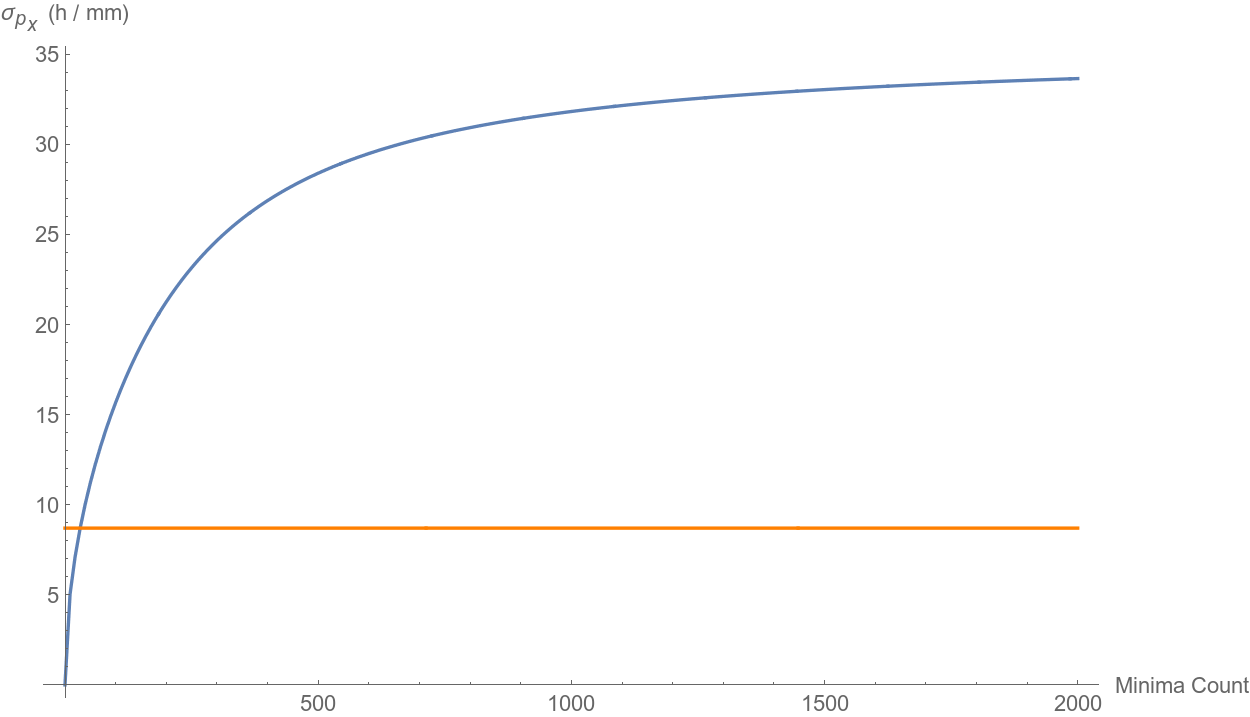
\includegraphics[height = 8cm]{stddev-convergence.png}
    \caption{
        Values used are for the \SI{0.2}{\milli\metre} slit case \\
        Blue: Convergence of \(\sigma_{p_x}\) \\
        Orange: Minimal value from Heisenberg's uncertainty principle
    }
    \label{fig:stddev-convergence}
\end{figure}

The left side of the \SI{0.1}{\milli\metre} slit fitted the theoretical pattern very well, though it didn't fit any of the secondary maxima on the right. This was very likely to be an equipment problem, since the proper pattern could be clearly seen with the naked eye while measuring it.

The entire measurement of the \SI{0.2}{\milli\metre} slit fitted the theoretical pattern quite well, though it was slightly wider than expected. This probably indicates the slit was actually a bit narrower than labelled. Indeed, when the theoretical pattern is replotted with a \SI{0.19}{\milli\metre} slit, it is in much better agreement all over.

The entire measurement of the \SI{0.4}{\milli\metre} slit, while having the correct general shape, doesn't fit very well, with the right side closest to fitting. Replotting with a \SI{0.38}{\milli\metre} slit fits the right side, but not the left. It is unknown what the cause of this is, but it might be the detector's hysteresis in moving the slit.

The distances between minima measurements in Table \ref{tab:minima} reflects this, with only the \SI{0.2}{\milli\metre} slit having the expected result to within error.

However, despite these issues, the shape of the patterns are close enough to match the Fraunhofer diffraction pattern reasonably.

Additionally, the respective \(\sigma_{p_x}\) of each measurement was more than four times the expected minimum value from Heisenberg's uncertainty principle. This is most likely due to only taking measurements for the middle five maxima, while in reality it has an infinite number of maxima of decreasing intensity.

Due to the mathematics of \(\sigma_{p_x}\) in the Fraunhofer diffraction pattern, convergence is very very slow (Figure \ref{fig:stddev-convergence}), with over 30 minima required to be measured to just to pass the minimum value imposed by the uncertainty principle, and over 5000 required to get within \SI{98}{\percent} of the real value.

This is impracticable, if not impossible, so therefore this is not a effective way to test Heisenberg's uncertainty principle.

\end{document}